\documentclass[uplatex]{jsarticle}
\usepackage{amsmath}
\usepackage{cite}
% hyperref (uplatex+dvipdfmx) + 日本語ブックマーク
\usepackage[dvipdfmx,unicode,bookmarks=true]{hyperref}
\usepackage{pxjahyper}
\hypersetup{
  colorlinks=true,
  linkcolor=blue,
  urlcolor=blue,
  citecolor=blue,
  bookmarksnumbered=true
}
\ifdefined\CI
  \PassOptionsToPackage{demo}{graphicx}
\fi
\usepackage{graphicx}

\title{こんにちは\LaTeX}
\author{山田太朗}
\date{\today}

\begin{document}

\maketitle

\section{はじめに}

GitHub Actions のCIを試しています。画像をダミーにしています。テスト4回目です。

\begin{figure}[htbp]
	\centering
	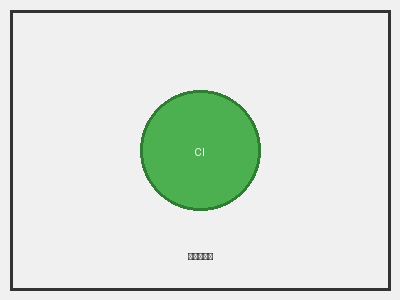
\includegraphics[width=0.6\textwidth]{figures/test-image}
	\caption{CIテスト用の画像}
	\label{fig:test-image}
\end{figure}

この画像はCI環境で正しく処理されるはずです。\cite{fujita2020}

\bibliographystyle{jplain}
\bibliography{refs}

\end{document}
